% Copyright (c) 2011 Martin Ueding <dev@martin-ueding.de>
%
\documentclass[12pt]{report}
\usepackage{geometry}
\geometry{a4paper, left=2cm, right=2cm, top=2cm, bottom=2cm}
\usepackage{graphicx}
\usepackage{amssymb}
\usepackage{amsmath}
\usepackage{epstopdf}
\usepackage[utf8]{inputenc}
\usepackage[activate]{pdfcprot}
\usepackage{setspace}
\usepackage[ngerman]{babel}
\usepackage[parfill]{parskip}
\usepackage{hyperref}
\usepackage{color}
\usepackage{units}
\definecolor{darkblue}{rgb}{0,0,.5}
\definecolor{lightblue}{rgb}{0.9,.9,1}
\definecolor{gray}{rgb}{.3,.3,.3}
\hypersetup{colorlinks=true, breaklinks=false, linkcolor=black, menucolor=black, urlcolor=darkblue}
\DeclareGraphicsRule{.tif}{png}{.png}{`convert #1 `dirname #1`/`basename #1 .tif`.png}

% Format for listings
\usepackage{calc}
\usepackage{caption}
\DeclareCaptionFont{white}{\color{white}}
\DeclareCaptionFormat{listing}{\colorbox{gray}{\parbox{\textwidth-2\fboxsep}{#1#2#3}}}
\captionsetup[lstlisting]{format=listing,labelfont=white,textfont=white, margin=0pt, font={bf,footnotesize}}
\usepackage[T1]{fontenc}
\usepackage[scaled]{beramono}
\usepackage{listings}
\lstset{
	breaklines=true,
		showstringspaces=false,
		framexleftmargin=0pt,
		framexrightmargin=0pt,
		framextopmargin=0pt,
		framexbottommargin=0pt,
		frame=b,
		xleftmargin=0pt,
		xrightmargin=0pt,
		basicstyle=\small\ttfamily,
		keywordstyle=\color{black}\bfseries,
		tabsize=4
}

% \code{language}{source file}{caption}{label}
\newcommand{\code}[4][]{\lstinputlisting[caption=#3, language=#1, label=#4]{#2}}

% Easy German quotes
\newcommand\gqq[1]{\glqq #1\grqq}

% Definition List Item
\newcommand\dd[2]{\item[\texttt{#1}] #2}

\newcommand\e[1]{\cdot 10^{#1}}

\title{EDV für Physiker}
\author{Martin Ueding \\ \href{mailto:mu@uni-bonn.de}{mu@uni-bonn.de}}

\begin{document}

\maketitle

\begin{abstract}
Bericht für die \gqq{EDV für Physiker und Physikerinnen} (physik130) Veranstaltung. Es wurden Einblicke in Linux, \LaTeX, C++ sowie ROOT vermittelt. Dieser Bericht enthält die Berichtsaufgaben.
\end{abstract}

\newpage

\tableofcontents
\newpage


\part{Linux}

\chapter{Übung 1}

\section{Befehle in der Konsole}
\label{commands}

\subsection{Benutzerverwaltung und -rechte}
\begin{itemize}
\dd{chmod}{Ändert Dateirechte.}
\dd{hostname}{Rechnername.}
\dd{last}{Letzte Anmeldungen aller Benutzer.}
\dd{ps}{Prozessliste.}
\dd{top}{Vorgänger von \texttt{htop}, eine interaktive Prozessverwaltung.}
\dd{uname}{Kernelversion, Rechnername, ...}
\dd{uptime}{Zeigt, wie viele Nächte der Rechner am Stück durchgemacht hat.}
\dd{whoami}{Eigener Benutzername.}
\dd{w}{Wie \texttt{who}, nur ausführlicher.}
\end{itemize}

\subsection{Dateibehandlung}
\begin{itemize}
\dd{bzip2}{Komprimiert eine Datei.}
\dd{cd}{Wechselt in das angegebene Verzeichnis. Dabei ist \texttt{..} das übergeordnete Verzeichnis. Wird als Verzeichnis \texttt{-} angegeben, kommt man in das vorherige Verzeichnis. \texttt{cd} ohne Verzeichnis wechselt in das Heimatverzeichnis\footnote{Meistens \texttt{/home/<benutzername>}.}.}
\dd{cp}{Kopiert Dateien.}
\dd{df}{Listet die Dateisysteme mit Belegungsangabe.}
\dd{du}{Zeigt die Größe von Dateien auf dem Datenträger an. Diese muss nicht unbedingt mit der Größe überstimmen, die \texttt{ls} anzeigt, da die Dateien in Blöcken organisiert sind.}
\dd{find}{Führt eine Dateisystemtraverse nach speziellen Suchvorgaben durch und zeigt standardmäßig alle Dateien und Ordner an.}
\dd{gzip}{Komprimiert eine Datei.}
\dd{ls}{Listet den Inhalt des angegebenen oder aktuellen Verzeichnisses auf. Dabei werden auch Informationen über Zugriffsrechte und Eigentümer, Größe und Änderungsdatum angezeigt, gibt man \texttt{-l} an.}
\dd{mkdir}{Erstellt ein Verzeichnis.}
\dd{mv}{Verschiebt Dateien, Umbenennen ist ein Spezialfall.}
\dd{rmdir}{Löscht leere Verzeichnisse.}
\dd{rm}{Löscht Dateien.}
\dd{scp}{Kopiert über SSH.}
\dd{tar}{Erstellt ein Archiv mehrerer Dateien. Mit \texttt{tar -xzf archiv.tar.gt datei1 datei2…}\cite{man-tar} erstellt man direkt ein komprimiertes Archiv mehrerer Dateien.}
\dd{touch}{Setzt das Änderungsdatum einer Datei auf den aktuellen Zeitpunkt und erzeugt die Datei, falls sie nicht existiert.}
\end{itemize}

\subsection{Informationen zu Programmen}
\begin{itemize}
\dd{apropos}{Unscharfe Suche nach Befehlen.}
\dd{man}{Zeigt Handbücher zu Programmen an.}
\dd{whatis}{Zeigt die erste Zeile des Handbuchs an.}
\end{itemize}

\subsection{Textdateien}
\begin{itemize}
\dd{diff}{Vergleicht Dateien miteinander.}
\dd{emacs}{Texteditor.}
\dd{grep}{Filtert Zeilen nach einem Suchmuster.}
\dd{head}{Zeigt die ersten n Zeilen einer Datei an.}
\dd{less}{Zeigt eine Datei an und erlaubt scrollen, suchen, springen. Es können viele Befehle aus \texttt{vi} (gg, G, /, j, k) benutzt werden.}
\dd{pdflatex}{Übersetzt ein \LaTeX\ Dokument in ein PDF.}
\dd{sort}{Sortiert Zeilen.}
\dd{tail}{Gegenstück zu \texttt{head}.}
\dd{uniq}{Spezialfall von \texttt{sort -u}}
\dd{vim}{Texteditor für Programmierer.}
\dd{wc}{Zählt Wörter, Zeilen, Buchstaben.}
\end{itemize}

\subsection{Bash built-ins}
\begin{itemize}
\dd{clear}{Fügt leere Zeilen ein, bis der Bildschirm leer ist.}
\dd{set}{Zeigt das Environment der Shell an.}
\dd{echo}{Gibt Text aus.}
\dd{history}{Zeigt die letzten Kommandos an.}
\end{itemize}

\subsection{Diverses}
\begin{itemize}
\dd{bc}{Einfacher Taschenrechner. Man sollte in der Bash allerdings nicht mit \texttt{\$(echo 5+4 | bc)} rechnen, sondern die neuen, von C übernommenen Funktionen zum direkten Rechnen, \texttt{\$((5+4))}, benutzen.}
\dd{blkid}{Zeigt die UUID der Partitionen an.}
\dd{e2label}{Zeigt und vergibt Partitionslabel.}
\dd{ssh}{Öffnete eine Shell auf einem anderen Computer.}
\dd{wget}{Lädt Dateien per http oder ftp.}
\dd{cal}{Zeigt einen Kalendermonat an.}
\dd{date}{Zeigt das Datum in einem gewählten Format an.}
\dd{gv}{Zeigt eine PDF oder PS Datei an. Normalerweise würde man okular (KDE) oder evince (Gnome) benutzen.}
\end{itemize}

\section{absoluter und relativer Pfad}

Ein absoluter Pfad beginnt immer mit einem \texttt{/}, wie beispielsweise \\ \texttt{/home/mu/Dokumente/Studium/EDV/Bericht} oder \texttt{/dev/null}. Ein relativer Pfad bezieht sich immer auf ein aktuelles Arbeitsverzeichnis. Beispielsweise beschreibt \texttt{datei.tex} die Datei \texttt{/tmp/datei.txt}, falls der Benutzer gerade \texttt{/tmp} als Arbeitsverzeichnis hat. Pfade können auch \texttt{..} enthalten, dies bezeichnet das übergeordnete Verzeichnis. Ist man gerade in \texttt{/etc/apache2}, so kann man mit \texttt{../passwd} auf die zentrale Passwortdatei verweisen.

Gemeinerweise können absolute Pfade auch \texttt{..} enthalten, so wäre \\
\texttt{/etc/apache2/../passwd} ein legaler Pfad, sinnvoll ist es in vielen Fällen allerdings nicht.

\section{grundlegende Emacs Steuerung}

\begin{table}[htb]
\begin{center}
\begin{tabular}{ll}
Aktion & Tasten \\
\hline
Cursor links & C-b \\
Cursor rauf & C-p \\
Cursor rechts & C-f \\
Cursor runter & C-n \\
Datei speichern & C-x C-s \\
Emacs beenden & C-x C-c \\
Hilfe aufrufen & C-h t \\
Seite rauf & M-v \\
Seite runter & C-v \\
\end{tabular}
\end{center}
\caption{Grundlegende Emacs Tastenkombinationen.}
\end{table}

\chapter{Übung 2}

Neue Befehle sind in §\ref{commands} mit den Befehlen aus vorherigen Übungen zusammen.

\section{Das Unix-Hilfe-System -- der \texttt{man} Befehl}

Generell sollte jedes Programm eine Handbuchseite haben, die genauso wie das Programm selbst heißt. So kann man mit \texttt{man Programm} diese Seite aufrufen.

Bash Builtins haben keine solche Hilfeseite, sie werden mit \texttt{help Kommando} dokumentiert, oder können in \texttt{bash.1} nachgeschaut werden.

Darüber hinaus gibt es noch die info Dokumente.

Meistens haben Programme auch noch eine eigene Hilfe dabei, die mit \texttt{Programm -h} oder \texttt{Programm --help} aufgerufen werden kann.

\section{Datums- und Kalenderangaben}

\section{Bash Variablen}

Mit \texttt{echo \${HOME}} kann man das Heimatverzeichnis anzeigen lassen. Dabei ist \texttt{echo \$HOME} eine der vielen Environmentvariablen, die in der Bash gesetzt sind. Man kann sie mit \texttt{set} anschauen. \texttt{echo \${HOSTNAME}} enthält den Rechnernamen.

Mit den geschweiften Klammern kann man mehrere Wörter aus einem erzeugen, dies ist praktisch für das erstellen von Sicherungskopien: \verb#cp foo{,.bak}# erstellt eine Kopie der Datei \texttt{foo} nach \texttt{foo.bak}, ohne dass man foo zweimal schreiben muss.

Das Programm \texttt{cal} zeigt einen Kalendermonat an. Der September 1752 ist etwas anders, als die restlichen Monate, da hier in einigen, leider nicht allen, Ländern der Wechsel zwischen Kalendersystemen vollzogen worden ist.

\section{Umgang mit Dateien und Verzeichnissen}

Hier gibt es wenig zu beschreiben, man muss sein aktuelles Arbeitsverzeichnis im Auge behalten und beachten, dass \texttt{rmdir} nur leere Verzeichnisse löscht.

\section{Absolute und relative Pfade}

Auch hier muss man sein Arbeitsverzeichnis für die relativen Pfade im Kopf haben, ansonsten ist es alles recht logisch.

\section{Wildcards}

Die Dateien lassen sich recht einfach mit dem Code aus Listing \ref{code:touch} erstellen. Dabei werden die geschweiften Klammern benutzt, um mehrere Dateien, die Namensbestandteile gemeinsam haben, zu erzeugen.

\begin{lstlisting}[caption=Anlegen der Dateien, language=bash, label=code:touch, float=htb]
touch datei{1..9}.txt logfile{10,10a,11,11a,11b}.txt
\end{lstlisting}

Listing \ref{code:ls} zeigt, wie man diese Dateien ausgeben (Ausgabe in Listing \ref{code:ls.out}) kann.

\lstinputlisting[caption=ls.sh, language=bash, label=code:ls, float=htb]{Uebung_02/wildcards/ls.sh}
\lstinputlisting[caption=Ausgabe von ls.sh, label=code:ls.out, float=htb]{Uebung_02/wildcards/ls.sh.out}

Ich habe hier \texttt{echo} anstelle von \texttt{ls} benutzt, da die Wildcards so oder so von der Bash und nicht vom Befehl aufgelöst werden und \texttt{ls} jede Datei auf eine eigene Zeile schreibt, sofern \texttt{STDOUT} kein Terminal ist. Dies spart ein klein wenig Platz und erzeugt letztlich die gleiche Ausgabe.

\section{Umgang mit Rechten unter Unix}

Jede Datei hat drei grundlegende Rechte, lesen (r), schreiben (w) und ausführen (x). Darüber hinaus gibt es noch drei Kategorien: Eigentümer, Gruppe und Alle. Mit \texttt{chmod -w} entzieht man allen das Schreibrecht, auch sich selbst. Setzt man die Rechte auf \texttt{rw-r--r--}\footnote{mit \texttt{chmod 644}} darf nur der Eigentümer die Datei schreiben, alle sie aber lesen.

\chapter{Übung 3}

\section{Weitere Unix-Befehle}

Siehe §\ref{commands}.

\section{Eingabe- und Ausgabeumleitung}

\lstinputlisting[caption=standardausgabe.txt, label=code:standardausgabe, float=htb]{Uebung_03/standardausgabe.txt}

\section{Handling von Textdateien}

Man kann es sich an dieser Stelle einfach machen und alle Kennzeichen rauswerfen, die mit einer Ziffer beginnen und es bleiben dann nur noch deutsche Kennzeichen übrig. Der Ansatz (Listing \ref{code:auto-einfach}) ist nicht nennenswert robust, erfüllt aber in der kleinen Eingabemenge seinen Zweck (Ausgabe in Listing \ref{code:auto-einfach.out}).

\lstinputlisting[caption=auto\_einfach.sh, label=code:auto-einfach, language=bash, float=htb]{Uebung_03/auto_einfach.sh}

\lstinputlisting[caption=Ausgabe von auto\_einfach.sh, label=code:auto-einfach.out, float=htb]{Uebung_03/auto_einfach.sh.out}

Allerdings ist es mit den Kennzeichen nicht so ganz einfach, möchte man wirklich nur deutsche Kennzeichen haben. Es gibt deutsche und Euro-Kennzeichen, alle Neuen sind Letztere. Die alten haben noch einen Bindestrich, die neuen nicht mehr. Außerdem dürfen in den alten die Buchstaben B, F, G, I, O und Q nicht vorkommen.\cite{wiki-kfz}

Es gilt das Muster \texttt{XXX XX 0000}, in jeder Gruppe können auch weniger Zeichen sein. Allerdings dürfen es maximal 8 Zeichen sein, solange es kein Saisonkennzeichen ist.

Das führt dazu, dass man im regulären Ausdruck (RegEx) nicht einfach 3, 2 und 4 Zeichen suche lassen kann, ansonsten würden Zeichenketten zugelassen, die 9 Zeichen lang sind. Somit muss man eine Fallunterscheidung benutzten. Darüber hinaus dürfen bei einem alten Kennzeichen -- erkennbar an dem Bindestrich -- einige Buchstaben im mittleren Feld nicht auftauchen. Der komplexe reguläre Ausdruck ist in Listing \ref{code:auto} gezeigt.

\lstinputlisting[caption=auto.sh, language=bash, label=code:auto, float=htb]{Uebung_03/auto.sh}

\lstinputlisting[caption=Ausgabe von auto.sh, label=code:auto.out, float=htb]{Uebung_03/auto.sh.out}

Man sieht, dass die gleiche Liste (Listing \ref{code:auto.out}) erzeugt wird, jedoch fällt das zweite Skript nicht auf diverse Gemeinheiten (Listing \ref{code:gemeinheiten}) rein, die man sich ausdenken könnte.

\begin{lstlisting}[caption=Gemeinheiten für Listing \ref{code:auto-einfach}, label=code:gemeinheiten, float=htb]
zKeinKennzeichen
NDH ND 2000
 1234 DC 75
@27
\end{lstlisting}

\section{Pipelines}
\subsection{Namen}
\lstinputlisting[caption=namen.dat, float=htb, label=code:namen.dat]{Uebung_03/namen.dat}

Es ist recht sinnfrei \texttt{cat} zu benutzen, um den Inhalt zu in \texttt{sort} zu bekommen, da \texttt{sort} die Datei auch selbst laden kann.

Mit dem entsprechenden Befehl (Listing \ref{code:namen}) bekommt man die gewünschte sortierte und gefiltere Ausgabe (Listing \ref{code:namen.out}) der Originaldatei (Listing \ref{code:namen.dat}).

\lstinputlisting[caption=namen.sh, language=bash, float=htb, label=code:namen]{Uebung_03/namen.sh}
\lstinputlisting[caption=Ausgabe von namen.sh, float=htb, label=code:namen.out]{Uebung_03/namen.sh.out}

\subsection{Zahlen}

\lstinputlisting[caption=zahlen.dat, float=htb, label=code:zahlen.dat]{Uebung_03/zahlen.dat}

Bei den Zahlen werden die Zahlen (Eingabedatei in Listing \ref{code:zahlen.dat}) exakt so sortiert, wie ich es erwarte. Und zwar nach ASCII Code Point. Es ist unnatürlich, dass eine 2 vor einer 1 steht, weil \textit{nach} der 1 eine weitere Zahl folgt. Da die Zahlen in der Datei allerdings ohne führende Nullen stehen, muss man die Zahl zuerst interpretieren, damit sie nach Zahlenwert sortiert werden kann. Dafür ist das \texttt{-n} Flag da. Der komplette Befehl ist in \ref{code:zahlen-sort} gezeigt. Die Ausgabe (Listing \ref{code:zahlen-sort.out}) ist wirklich nach Zahlenwert sortiert.

\lstinputlisting[caption=zahlen-sort.sh, float=htb, label=code:zahlen-sort]{Uebung_03/zahlen-sort.sh}
\lstinputlisting[caption=Ausgabe von zahlen-sort.sh, float=htb, label=code:zahlen-sort.out]{Uebung_03/zahlen-sort.sh.out}

\section{Komprimierung und Archivierung}

Leider war die Datei \texttt{cc++.tar} zum Bearbeitungszeitpunkt nicht verfügbar. So habe ich $\unit[55]{MiB}$ HTML Dateien zum Testen benutzt.

\begin{table}[h!]
\begin{center}
\begin{tabular}{llll}
\label{table:compression-results}
Programm & Option & Zeit [s] & Dateigröße [KiB] \\
\hline
tar + bzip2 &  & 4.29 + 11.02 & 12701 \\
tar + bzip2 & -1 & 4.29 + 11.81 & 12701 \\
tar + bzip2 & -9 & 4.29 + 11.00 & 12701 \\
tar + gzip &  & 4.29 + 2.37 & 14149 \\
tar + gzip & -1 & 4.29 + 1.51 & 15514 \\
tar + gzip & -9 & 4.29 + 4.30 & 14073 \\
zip &  & 2.29 & 16694\\
\end{tabular}
\end{center}
\caption{Zeiten und Dateigrößen verschiedener Kompressionsprogramme}
\end{table}

Man sieht an den Daten in Tabelle \ref{table:compression-results}, dass bzip2 etwas besser komprimiert, allerdings deutlich länger braucht. Zip ist am schnellsten, schafft allerdings auch am wenigsten Kompression.

Zip komprimiert jede Datei einzeln und kann so Passagen, die in mehreren Dateien vorkommen, nicht effizient komprimieren. Jedoch können einzelne Dateien aus dem Archiv genommen werden, bei einem komprimierten tar muss erst alles expandiert werden, damit eine einzelne Datei entnommen werden kann.

Das Skript, das die Zeiten misst, kann in §\ref{listing:compression} gefunden werden.


\section{Verteiltes Arbeiten}

Die Dateien auf den zwei verschiedenen Rechnern, die allerdings ihr Heimatverzeichnis teilen, ist fast gleich, bis auf die Datei, die auf dem anderen Rechner schon erstellt worden ist.

Kopiert man die Dateien auf einen Rechner, kann man sie mit \texttt{diff -u} vergleichen. Die Unterschiede sind Listing \ref{code:diff} gezeigt.

\begin{lstlisting}[caption=Unterschied zwischen Ordnerinhalten, float=htb, label=code:diff]
--- ls-lR.host1 2011-10-30 14:43:46.031286114 +0100
+++ ls-lR.host2 2011-10-30 14:43:49.275286307 +0100
@@ -2 +2 @@
-insgesamt 156
+insgesamt 184
@@ -9 +9,2 @@
--rw-r--r-- 1 ueding studis      0 30. Okt 2011  ls-lR.host1
+-rw-r--r-- 1 ueding studis  24614 30. Okt 2011  ls-lR.host1
+-rw-r--r-- 1 ueding studis      0 30. Okt 2011  ls-lR.host2
\end{lstlisting}

Die Datei, in die die Ausgabe umgeleitet wird, wird zwar direkt angelegt, weil bash sie öffnet, allerdings hat sie noch keine Größe. Erst nach dem Durchlauf ist die Datei komplett da. Zwischen Physik und Astro CIP-Pool sind natürlich alle Dateien anders, weil es komplett verschiedene Ordner sind. Nur Dateien wie meine \texttt{.bashrc} sind beispielsweise auf beiden Seiten vorhanden und haben die gleiche Größe, jedoch unterscheidet sich das Änderungsdatum.

\section{Shell - Skript}

Für die Farben kann man eine einfache \texttt{for}-Schleife benutzen, wie in Listing \ref{code:farben} gezeigt. Dies erzeugt die gewünschte Ausgabe (Listing \ref{code:farben.out}).

\lstinputlisting[caption=farben.sh, language=bash, float=htb, label=code:farben]{Uebung_03/farben.sh}

\lstinputlisting[caption=Ausgabe von farben.sh, float=htb, label=code:farben.out]{Uebung_03/farben.sh.out}


\subsection{Zahlen}

Für die Zahlen kann man entweder \texttt{{1..3}} benutzen\footnote{Ein Beispiel für die \texttt{{1..3}} finden Sie in §\ref{listing:zahlen2}}, oder eine C-artige for-Schleife benutzen (Listing \ref{code:zahlen}, Ausgabe in Listing \ref{code:zahlen.out}). Die Syntax, die auf dem Übungszettel steht, gibt es nicht, ich weiß nicht, wie Sie die Ausgabe auf dem Übungszettel damit erzeugt haben.

\lstinputlisting[caption=zahlen.sh, language=bash, label=code:zahlen, float=htb]{Uebung_03/zahlen.sh}
\lstinputlisting[caption=Ausgabe von zahlen.sh, label=code:zahlen.out, float=htb]{Uebung_03/zahlen.sh.out}

Soll von 2 bis 20 gezählt werden und der Vorname ausgegeben werden, wenn der Zähler auf 10 steht, sieht das Skript so aus wie in Listing \ref{code:zahlen-name}. (Ausgabe in Listing \ref{code:zahlen-name.out}.)

\lstinputlisting[caption=zahlen\_name.sh, language=bash, label=code:zahlen-name, float=htb]{Uebung_03/zahlen_name.sh}
\lstinputlisting[caption=Ausgabe von zahlen\_name.sh, label=code:zahlen-name.out, float=htb]{Uebung_03/zahlen_name.sh.out}

\section{Analyse von Pipelines}

Der Befehl \verb#find /uebung_03 -type f -exec du -k {} \;| sort -n -r#\ iteriert durch das Verzeichnis \verb#uebung_03# und dessen Unterverzeichnisse, sucht Einträge heraus, die Dateien sind (und keine Ordner, Links, Fifos, …). Auf jede dieser Dateien wird der Befehl \texttt{du -k} ausgeführt. Man erhält eine Liste mit Dateigrößen in kiB. Diese Liste wird dann numerisch und rückwärts sortiert, also die größten Dateien nach vorne.

\subsection{Teilaufgabe a}
In dieser Aufgabe ist wahrscheinlich ein \verb#ps aux | grep ueding# gefragt. Dies ist allerdings gefährlich, falls jemand anderes ein Programm ausführt, das meinen Namen im Namen hat, oder jemand anders so heißt wie ich, nur mit einer 2 dahinter. Außerdem wird \texttt{grep} auch sich selbst in der Ausgabe von \texttt{ps} finden, weil mein Name auch Teil des Kommandos ist und somit dieser wieder in der Prozessliste auftaucht. Daher wäre es mit einer genauen Suche nach der Position in der Zeile etwas sicherer (Listing \ref{code:psauxgrep-beginning}). So hätte man beide Probleme aus dem Weg.

Allerdings kann man auch einfach das \texttt{a} weglassen und erhält direkt eine Liste mit seinen eigenen Prozessen und vermeidet an dieser Stelle die Benutzung von \texttt{grep} komplett.

\begin{lstlisting}[caption=Einschänkung des Suchbereichs, float=htb, label=code:psauxgrep-beginning]
ps aux | grep '^ueding '
\end{lstlisting}

\subsection{Teilaufgabe b}
Für das Sortieren hat \texttt{ps} auch eine entsprechende Option: \texttt{O+p}. So lässt sich mit \texttt{ps ux O+p} direkt nach Prozess-ID sortieren.

\subsection{Teilaufgabe c}
Mit \verb#ps ux O+p > myprocesses.txt# lässt sich die entsprechende Datei (Listing \ref{code:myprocesses}) erzeugen.

\lstinputlisting[caption=myprocesses.txt, label=code:myprocesses, float=htb]{Uebung_03/myprocesses.txt} 


Wenn man mag, kann man natürlich auch den Code aus Listing \ref{code:chain-pipe} benutzen.

\begin{lstlisting}[caption=verkettete Pipes, label=code:chain-pipe, float=htb]
ps aux | grep ueding | sort -n > myprocesses.txt
\end{lstlisting}

% Copyright (c) 2011 Martin Ueding <dev@martin-ueding.de>

\part{\LaTeX}

\chapter{Übung 4}

\textbf{Faust - Der Tragödie erster Teil, Johann Wolfgang von Goethe}

Quelle: \url{http://de.wikisource.org/}

\[ \cdots \]

\textbf{Faust.} \\
Das also war des Pudels Kern! \\
Ein fahrender Scolast? Der Casus macht mich lachen. \\

\begin{flushright}
\textbf{Mephistopheles.} \\
\textit{Ich salutire den gelehrten Herrn! \\
Ihr habt mich weidlich schwitzen machen.}
\end{flushright}

\textbf{Faust.} \\
Wie nennst du dich?

\begin{flushright}
\textbf{Mephistopheles.}
\textit{Die Frage scheint mir klein, \\
Für einen, der das Wort so sehr verachtet, \\
Der, weit entfernt von allem Schein, \\
Nur in der Wesen Tiefe trachtet.}
\end{flushright}

\textbf{Faust.} \\
Bey euch, ihr Herrn, kann man das Wesen \\
Gewöhnlich aus dem Namen lesen, \\
Wo es sich allzu deutlich weist, \\
Wenn man euch Fliegengott, Verderber, Lügner heit. \\
Nun gut wer bist du denn?

\begin{flushright}
\textbf{Mephistopheles.} \\
\textit{Ein Theil von jener Kraft, \\
Die stets das Böse will und stets das Gute schafft.}
\end{flushright}

\[ \cdots \]


\chapter{Übung 5}

\section{Mathematischer Formelsatz}

\subsection{Beispiele auf Aufgabenblatt}

\paragraph{Fließtext}
$a^2 + b^2 = c^2$

\paragraph{eckige Klammern}
\[ a^2 + b^2 = c^2 \]

\paragraph{equation Umgebung}
\begin{equation}
a^2 + b^2 = c^2
\end{equation}

%\paragraph{equation* Umbebung}
%\begin{equation*}
%a^2 + b^2 = c^2
%\end{equation*}

\subsection{matheuebung.pdf}

\subsubsection{Gleichungsumformungen}

\paragraph{Erstes Beispiel (Einfache Gleichung}
\begin{equation}
4x^2 + 2xv + v^2 = (2x + v)^2 - 2xv
\end{equation}

\paragraph{Zweites Beispiel (Gleichung über mehrere Zeilen)}
\begin{eqnarray}
(2x + 1)(2x - 1) &=& 7 \nonumber \\
4x^2 - 1 &=& 7 \nonumber \\
x^2 &=& 2  \nonumber\\
x &=& \pm 2
\end{eqnarray}
\paragraph{Drittes Beispiel (Hochstellung, Wurzeln)}
\begin{eqnarray}
\left( a^{\frac{p}{q}} \right)^{rq} &=& \left( \left( \sqrt[q]{a^p} \right)^q \right)^r \nonumber \\
&=& (a^p)^r = a^{rp}
\end{eqnarray}
\paragraph{Viertes Beispiel (Brüche)}
\begin{equation}
\frac{1-x^4}{(x^3)^2}-\left(\frac{1}{x}\right)^2=\frac{1-2x^4}{x^6}
\end{equation}

\paragraph{Fünftes Beispiel (Mathe im Fließtext )}
\begin{equation}
m=\frac{v^2r}{G}
\end{equation}
Mit $G = \unitfrac[6{,}67 \e{-11}]{Nm^2}{kg^2}$, $v = \unitfrac[29{,}77]{km}{s}$ und $r = \unit[1{,}49570 \e{8}]{km}$ ergibt
sich für die Masse $M$ der Sonne:
\begin{equation}
M = \frac
	{\left(\unitfrac[22{,}77 \e{3}]{m}{s} \right)^2 \cdot \unit[1{,}49570 \e{11}]{m}}
	{\unitfrac[6{,}67 \e{-11}]{Nm^2}{kg^2}}
= \unit[1{,}98 \e{30}]{kg}
\end{equation}

\paragraph{Sechstes Beispiel (Klammerausdruck, Array)}
\begin{eqnarray}
\ln(1+|u|) &=& x-c \nonumber \\
1+|u| &=& e^{x-c} \nonumber \\
|u| &=& e^{x-c}-1 \nonumber \\
u(x) &=& \begin{cases}
e^{x-c}-1 & \text{für} \, x > c \\
0 & \text{für}\, x=c \\
-e^{x-c}+1 & \text{für} \, x < c
\end{cases}
\end{eqnarray}

\paragraph{Siebtes Beispiel (Funktionen, verschachtelte Brüche)}
Aus der l’Hos\-pi\-tal\-schen Regel folgt:

\[
\lim_{x \rightarrow \infty} \frac{\ln\sin(\pi x)}{\ln\sin(x)} =
\lim_{x \rightarrow \infty} \frac
	{\pi \frac{\cos(\pi x)}{\sin(\pi x)}}
	{\frac{\cos(x)}{\sin(x)}} =
\lim_{x \rightarrow \infty} \frac{\pi \tan(x)}{\tan(\pi x)} =
\lim_{x \rightarrow \infty} \frac{\pi / \cos^2(x)}{\pi / \cos^2(\pi x)} =
\lim_{x \rightarrow \infty} \frac{\cos^2(\pi x)}{\cos^2(x)} =
1
\]

\subsubsection{Die Lösung von Integralen (Integrale)}
\begin{equation}
f(x)=\int_a^b \frac{3x^2}{x^3-1} \mathrm dx
\end{equation}

Exkurs:

\begin{align}
u &:= x^3-1 \nonumber \\
\frac{\mathrm dx}{\mathrm dy} &= 3x^2 \nonumber \\
\mathrm dx &= \frac{\mathrm du}{3x^2} \nonumber \\
\int \frac{3x^2}{x^3-1} \mathrm dx &= \int \frac{1}{u} \mathrm du \\
f(x) &= \ln(|u|) + c
\end{align}

Es folgt damit:

\[ f(x) = [\ln(x^3-1)]_a^b \]

\paragraph{Die Integral - Multiplikationsregel}

Es gilt:

\[ \int_a^b g'(x)f(x)\mathrm dx = [g(x)f(x)]_a^b - \int_a^b g(x)f'(x)\mathrm dx \]

Berechnen wir damit als Beispiel das Integral $\int \ln(x) \mathrm dx = \int 1 \cdot \ln(x) \mathrm dx$!
\textbf{Führen Sie die Berechnung des Integrals in diesem Dokument zu Ende!}\footnote{Falls dies an mich gerichtet sein sollte, beißt sich das mit der Aufgabenstellung, dass man das Dokument möglichst wie im Original nachbauen soll.}

\subsection{Vektoren und Matrizen (Vektoren, Arrays, Fortsetzungspunkte)}

Der Winkel $\alpha$ zwischen zwei Vektoren $\vec{a}$ und $\vec{b}$ ist gegen durch:

\[ \cos(\alpha) = \frac{\vec{a} \cdot \vec{b}}{|\vec{a}| \cdot |\vec{b}|} \]

Ein lineares Gleichungssystem $A \cdot x = b$, wobei $A = (A_{ij})_{n \times n}$ eine $n \times n$ Matrix und $x=(x_i)_n$ und $b=(b_i)_n$ Vektoren mit $n$ Elementen sind, sieht ausgeschrieben so aus:

\[
\left(
\begin{matrix}
a_{11} & a_{12} & \cdots & a_{1n} \\
a_{21} & a_{22} & \cdots & a_{2n} \\
\vdots & \vdots & \ddots & \vdots \\
a_{n1} & a_{n2} & \cdots & a_{nn} \\
\end{matrix}
\right)
\left(
\begin{matrix}
a_{x_1}  \\
a_{x_2}  \\
\vdots \\
a_{x_n}  \\
\end{matrix}
\right)
=
\left(
\begin{matrix}
a_{b_1}  \\
a_{b_2}  \\
\vdots \\
a_{b_n}  \\
\end{matrix}
\right)
\]

Die Summenschreibweise für die $i$-te Zeile dieser Matrix ist dann:

\[ \sum_{m=1}^n a_{im} \cdot x_m = b_i \]

\section{Einbindung von Graphiken}
Siehe \url{Uebung_05/Uebung05_Zubehoer/gesellschaft_vierte.pdf}.

\section{Weiteres zur Textstrukturierung}
Anstelle die Datei \texttt{gliederung.tex} zu formatieren, habe ich Verweise in diesen Bericht eingebracht, wo diese durchaus nützlich sein können.

Ein Anhang mit Code Listings ist auch schon vorhanden. Inzwischen habe ich die Anhänge in die jeweiligen Teile gepackt, somit habe ich momentan keine appendix-Umgebung am Ende.

Ein Inhaltsverzeichnis hat dieses Dokument natürlich auch.

Auf der Titelseite habe ich allerdings nur einen Autor. Würde man zwei haben wollen, kann man sie mit \verb#\\# trennen, so wie überall sonst auch.

Das Literaturverzeichnis habe ich diesem Artikel hinzugefügt.

\section{Berichtaufgaben}

Die Linuxbefehle (§\ref{commands}) habe ich als \texttt{itemize} gehalten, was ich übersichtlicher finde. Eine Tabelle kann als Tabelle \ref{table:compression-results} auf Seite \pageref{table:compression-results} gefunden werden. Diese Tabelle hat schon ein Label.

% Copyright (c) 2011 Martin Ueding <dev@martin-ueding.de>

\part{C++}

\section{Heron}

Der Algorithmus ist recht einfach umzusetzen, man benötigt die Formel, die auf dem Übungsblatt angegeben ist.

\begin{equation}
x_{n+1}=\frac{x_n+\frac{a}{x_n}}{2}
\end{equation}

Dabei ist $a$ die Zahl, von der die Wurzel bestimmt werden soll. Diese Formel braucht noch ein $x_0$, damit sie funktioniert. Hier kann man einfach jede beliebige Zahl benutzen. Allerdings ist $x_0=a$ keine allzu schlechte Wahl.

Eine Abbruchbedingung kann verschieden aussehen. Man kann nach einer gewissen Anzahl von Iterationen abbrechen. Ich habe mich dafür entschieden, abzubrechen, sobald sich die Zahl nur noch wenig verändert. Dazu muss man sich merken, welchen Wert die Zahl vorher hatte, um vergleichen zu können.

Das ganze Programm könnte man rekursiv implementieren, allerdings spricht hier nichts gegen eine iterative Variante, daher habe ich mich für letzteres entschieden. Mein Programm ist in Listing \ref{code:heron} zu sehen.

\code[c++]{Uebung_06/heron/heron.cpp}{heron.cpp}{code:heron}

Ich lasse $\sqrt{2} \approx 1.41421356237309504880168872421$\footnote{Mit \texttt{N[Sqrt[2], 30]} in Mathematica berechnet.} berechnen, die Ausgabe ist in Listing \ref{code:heron.2.out} zu sehen. Man kann sehen, dass das Programm schnell zu einem brauchbaren Ergebnis kommt, der Algorithmus also leistungsfähig ist.

\code{Uebung_06/heron/heron.2.out}{Ausgabe von heron für 2}{code:heron.2.out}
\code{Uebung_06/heron/heron.4.out}{Ausgabe von heron für 4}{code:heron.4.out}
\code{Uebung_06/heron/heron.10.out}{Ausgabe von heron für 10}{code:heron.10.out}

Für die CppDoc Kommentare habe ich in \cite{cppdoc} nachgeschaut.

\chapter{Übung 8}

\section{Berichtsaufgabe}

Das hier war noch auf den Aufgabenzetteln als Berichtsaufgabe gekennzeichnet, allerdings taucht es nicht in der finalen Liste auf:

Dieses Programm fügt mehrere Kommandozeilenargumente in eine Datei zusammen.

\code[c++]{Uebung_08/Consolidator/main.cpp}{Consolidator main.cpp}{code:consolidator-main.cpp}

\chapter{Übung 9}

\section{Versuchsergebnisse, die Zweite}

Dies ist das Programm aus der 7. Übung, entsprechend für die Berichtsaufgabe angepasst.

Bei der Bestimmung des Fehlers von $R$ weiß ich nicht genau, was $\delta R$ sein soll. Ich rechne jetzt mit

\begin{equation}
\Delta R = \sqrt{(\Delta U)^2 + (\Delta I)^2}
\end{equation}

\code[c++]{Uebung_09/bericht/bericht.cpp}{bericht.cpp}{}
\code{Uebung_09/bericht/bericht.out}{Ausgabedatei von bericht}{}
\code{Uebung_09/bericht/means.dat}{Ausgabe von bericht}{}

% Copyright (c) 2011 Martin Ueding <dev@martin-ueding.de>

\part{ROOT}

\chapter{Übung 10}

\begin{figure}[h]
\begin{center}
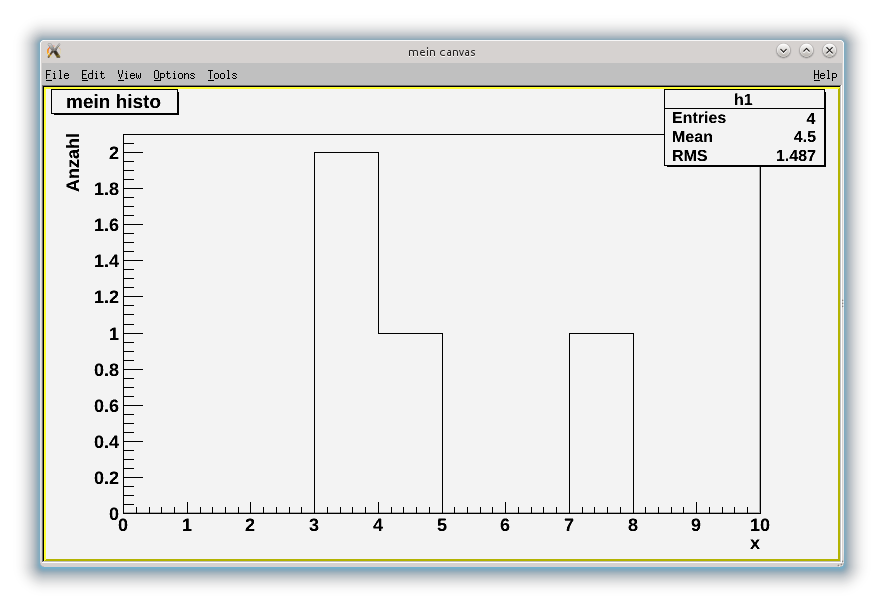
\includegraphics[width=10cm]{Uebung_10/default.png}
\caption{Standardplot}
\end{center}
\end{figure}



\begin{figure}[h]
\begin{center}
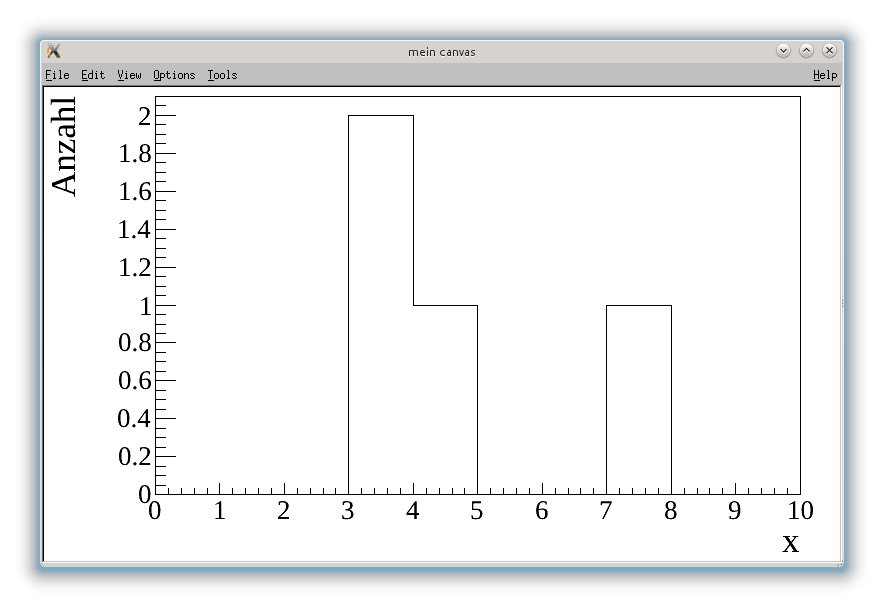
\includegraphics[width=10cm]{Uebung_10/babar.png}
\caption{BABAR Plot}
\end{center}
\end{figure}

Man kann mit \texttt{c1->SetLogx(1)} eine logarithmische Achse aktivieren und mit \texttt{c1->SetLogx(0)} wieder zurück zur linearen Achse wechseln.

\section{Berichtsaufgabe}

Man kann hier einfach den entsprechenden Konstruktor benutzen, da die Datei freundlichweise schon passend formatiert ist.

\code[c++]{Uebung_10/bericht.C}{Code für Plot}{code:root1}

ROOT gibt dann folgende Parameter für den Fit aus (Tablle \ref{table:fit}).

\begin{table}[h]
\begin{center}
\begin{tabular}{lcrcr}
Chi2 & = & $48.4851$ &  \\ 
NDf & = & $17$ &  \\ 
p0 & = & $-0.153455$ & $\pm$ & $0.0434887$ \\ 
p1 & = & $2.04459$ & $\pm$ & $0.00707916$ \\ 
\end{tabular} 
\caption{Parameter des Fits}
\label{table:fit}
\end{center}
\end{table}

ROOT zeichnet auch direkt die Linie ein. Man kann ihr Erscheinungsbild in der GUI dann auch noch verändern.


\begin{figure}[h]
\begin{center}
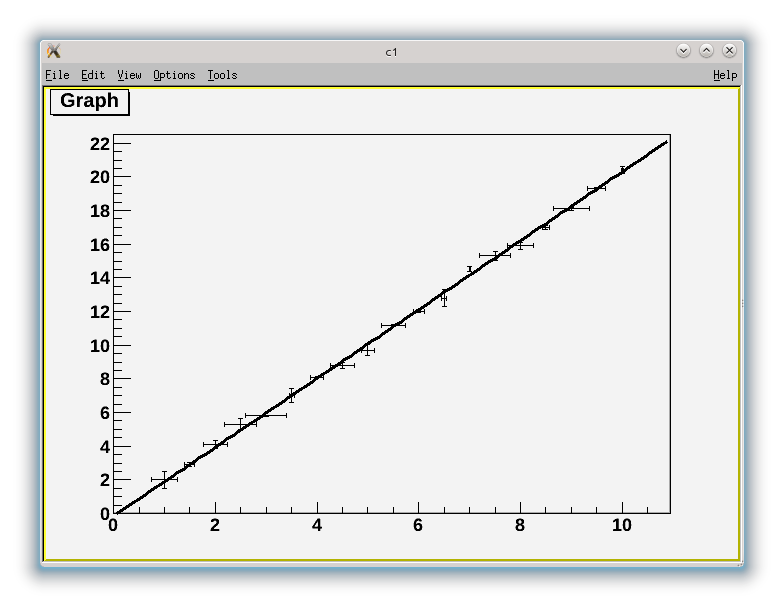
\includegraphics[width=10cm]{Uebung_10/fit.png}
\caption{Messwerte mit linearem Fit}
\end{center}
\end{figure}


\part{Anhang}

\lstlistoflistings

\begin{thebibliography}{n}
\bibitem{man-tar} Manual Page von \texttt{tar}.
\bibitem{wiki-kfz} \gqq{Kfz-Kennzeichen}, deutsche Wikipedia \url{https://secure.wikimedia.org/wikipedia/de/wiki/Kfz-Kennzeichen_\%28Deutschland\%29}
\bibitem{ritchie} Kerningham und Ritchie: \gqq{Programmieren in C}
\bibitem{cppdoc} \url{http://www.cppdoc.com/cppdoc_help.html}
\bibitem{rootbeginner} \url{hadron.physics.fsu.edu/~skpark/document/ROOT/root_beginers/ROOT_for_beginners_Day1.pdf}
\bibitem{wikilatex} \url{http://en.wikibooks.org/wiki/LaTeX/Tables}
\bibitem{root-pdf} \url{http://phacker.org/2009/02/20/minimal-program-to-create-histograms-from-a-file-with-root/}
\bibitem{latexspace} \url{http://www.maths.tcd.ie/~dwilkins/LaTeXPrimer/WhiteSpace.html}
\end{thebibliography}

\newpage

\chapter*{Erklärung}

Hiermit versichere ich, dass ich den vorliegenden Bericht selbstständig angefertigt, und nur die angegebenen Hilfsmittel benutzt habe.

\vspace{2cm}

\begin{tabular*}{0.75\textwidth}{@{\extracolsep{\fill}} l l l }
& 2439532 & \\
\hline
Ort/Datum & Martrikelnummer & Unterschrift
\end{tabular*}

\end{document}
